\section{System Demonstration}
\label{sec-demo}

\begin{figure*}[tp]
\centering
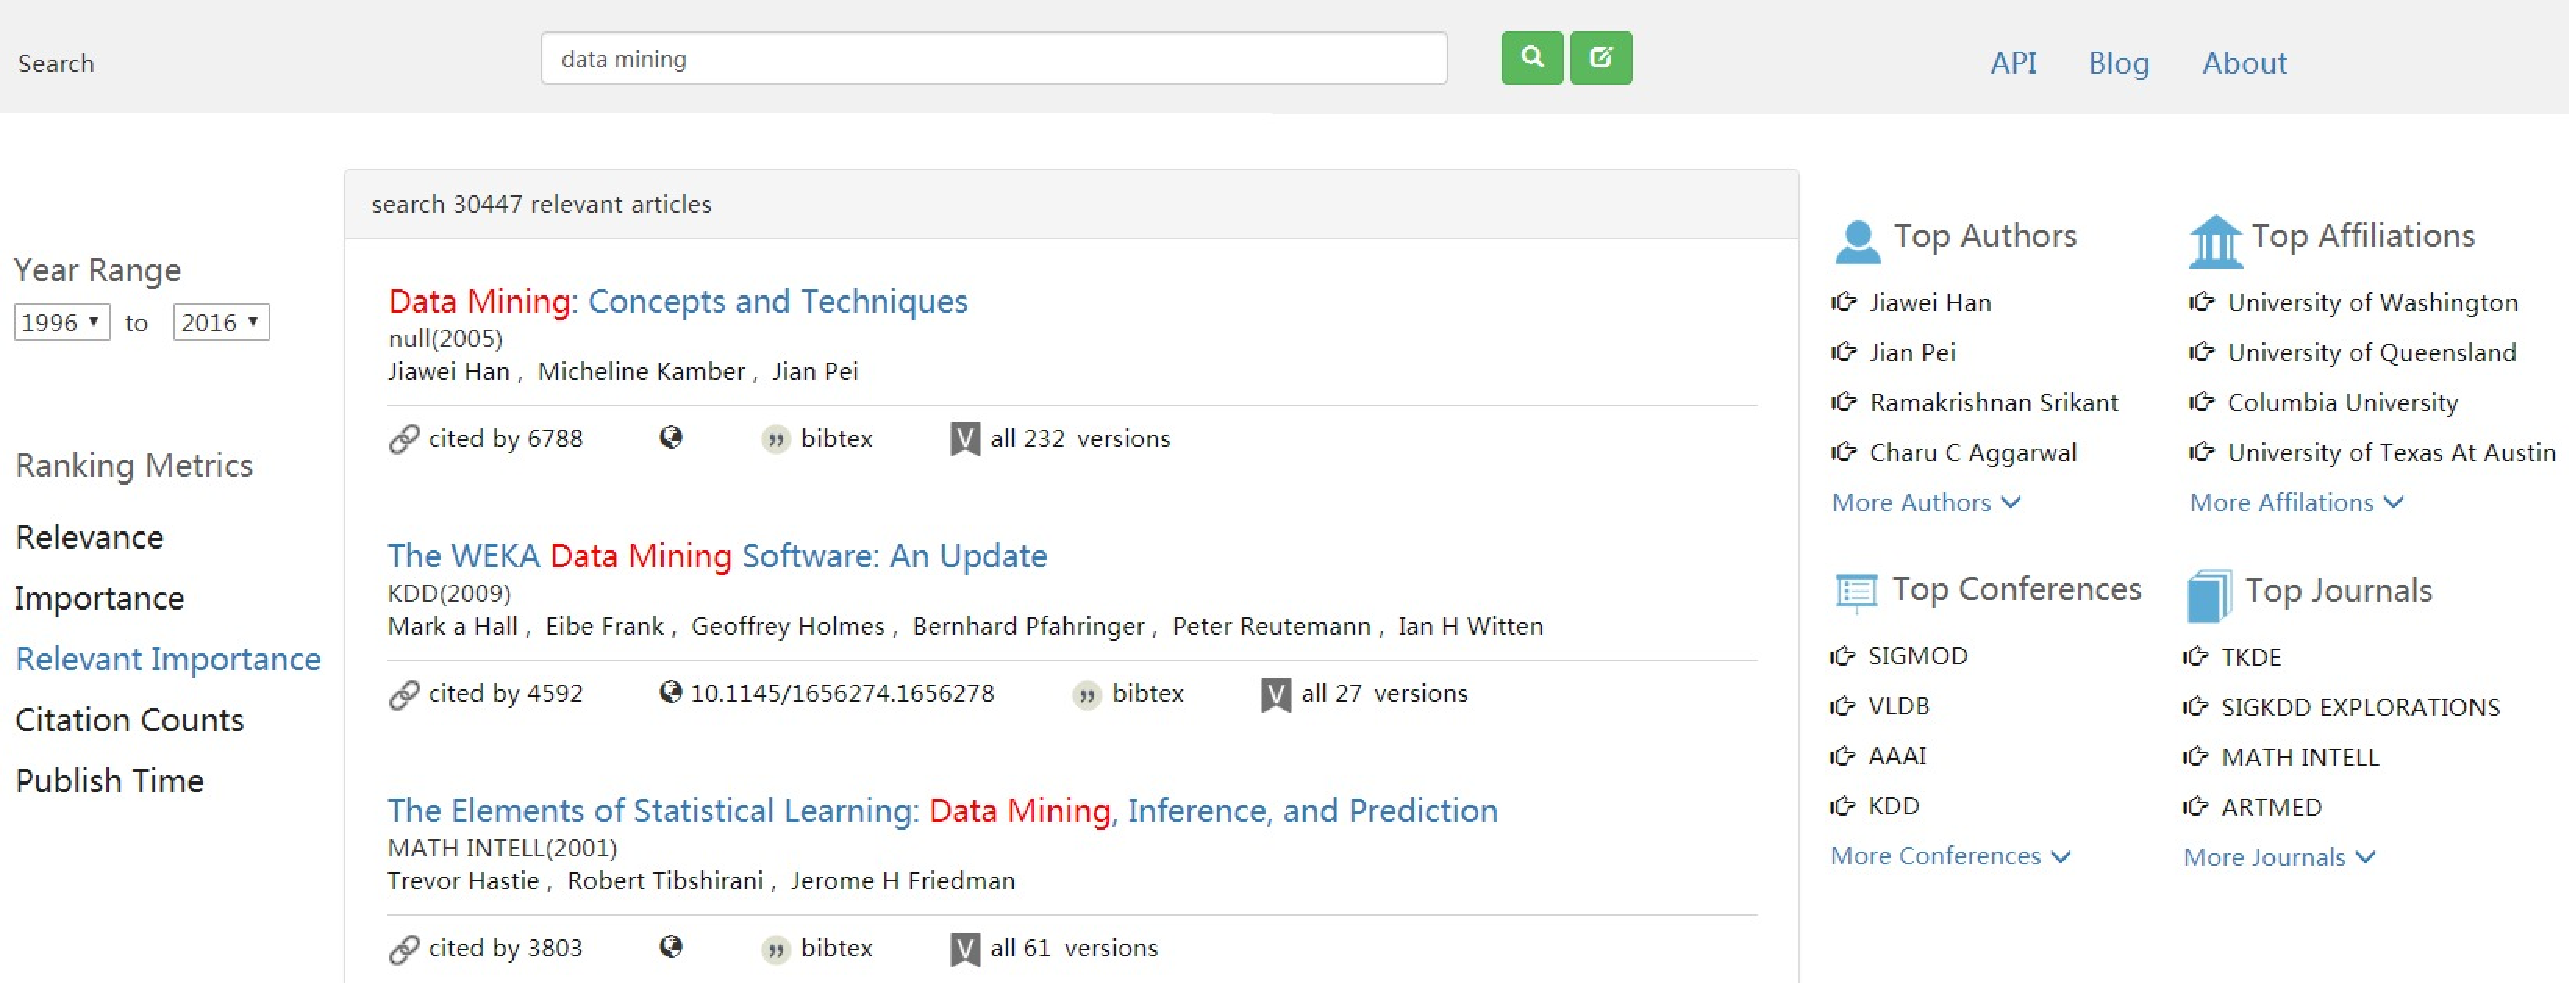
\includegraphics[width=\textwidth]{searchKeywords.pdf}
\caption{Search Keywords And Heterogeneous Entity Ranking}
\label{fig:searchKeywords}
\vspace{-3ex}
\end{figure*}

\begin{figure}
\centering
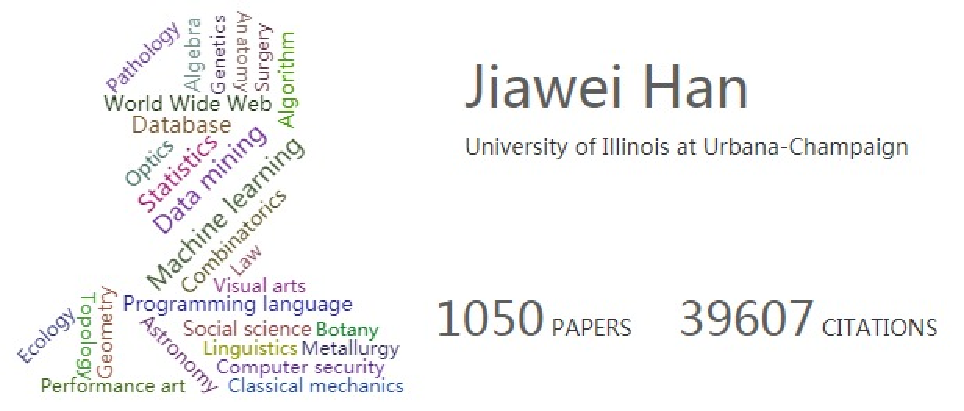
\includegraphics[width=\columnwidth]{hjwAvatar.pdf}
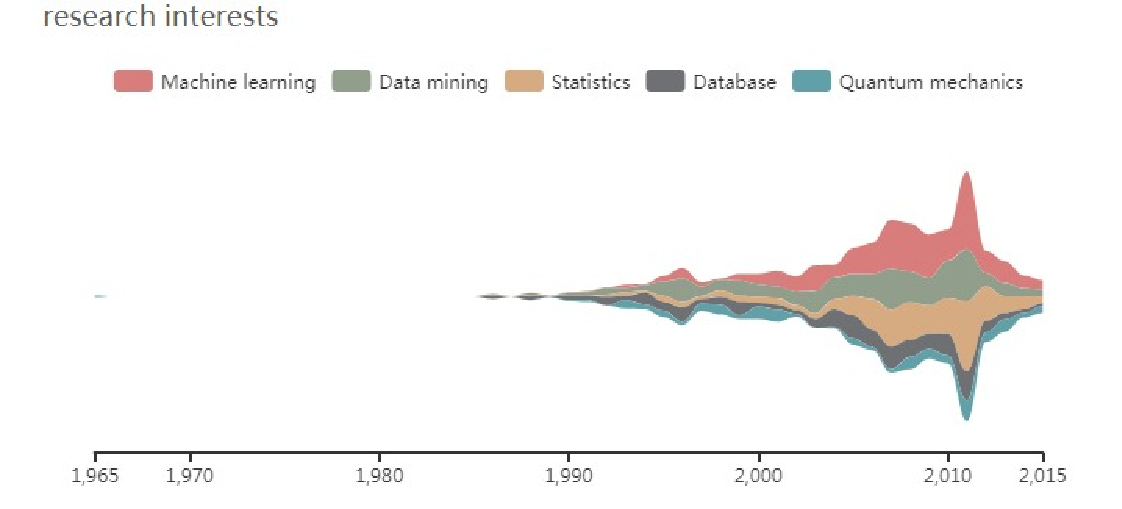
\includegraphics[width=\columnwidth]{hjwInterest.pdf}
%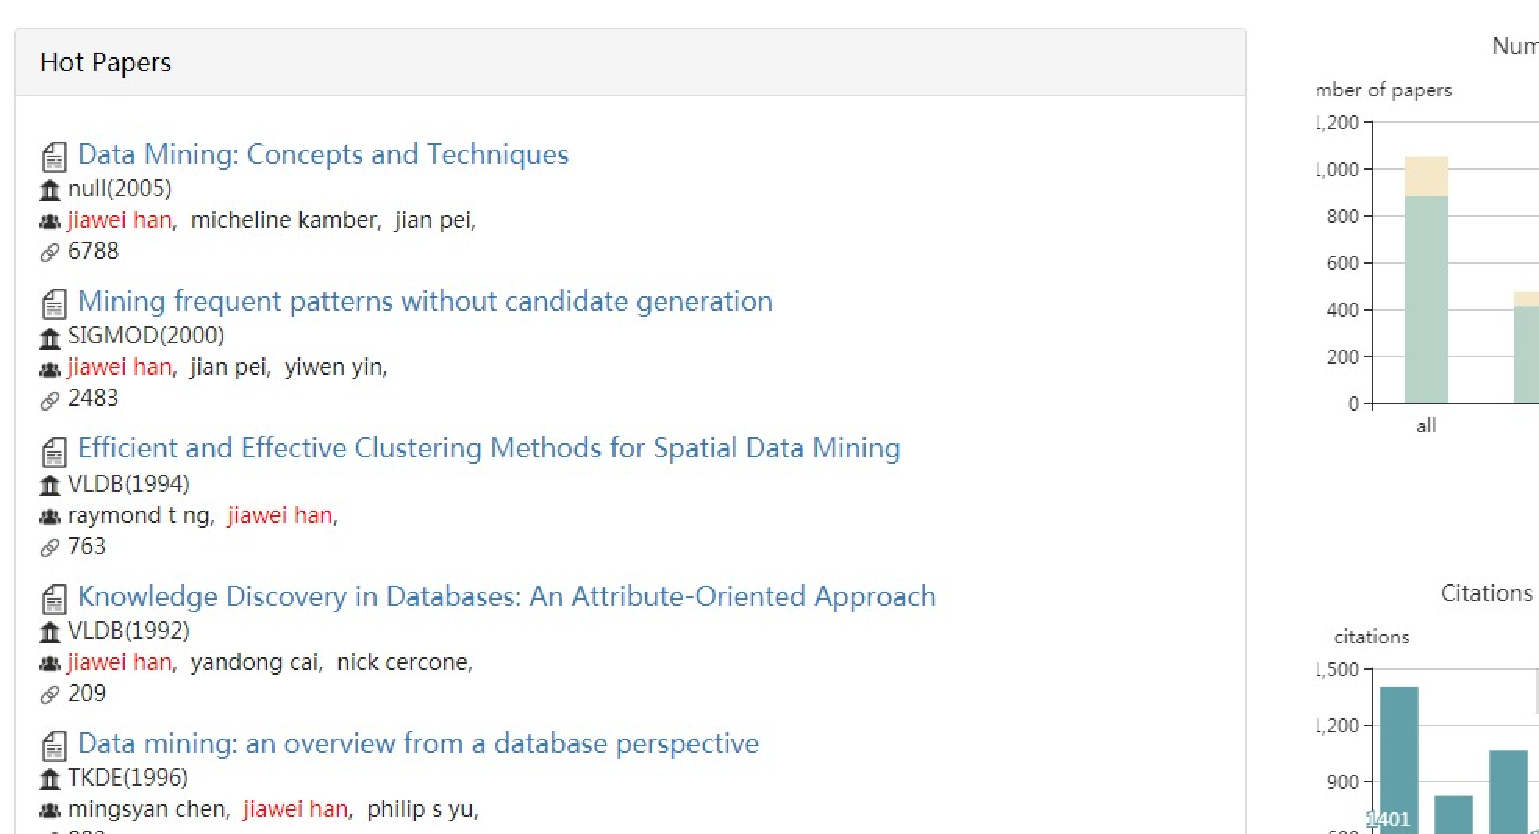
\includegraphics[width=\columnwidth]{hjwPapers.pdf}
\caption{Author Profiling}
\label{fig:hjwProfile}
\vspace{-3ex}
\end{figure}


The demonstration consists of three parts. (1) We walk through its various ranking metrics to demonstrate \oursystem on querying and heterogeneous entities ranking. (2) To further illustrate the profiling function based on scholarly data analysis, we take author profiling as an example. (3) Compared with MySQL, query performance has been significantly improved when utilizes Neo4j.
% heterogeneous entities ranking, ranking metrics
% author profiling
% storage advantage

\stitle{Querying and Ranking Scholarly Entity.} We demonstrate how to query and employ different ranking metrics to rank articles, as shown in Fig. \ref{fig:searchKeywords}. Moreover, We use heterogeneous scholarly entities ranking for deep scholarly data analysis.

\par
\oursystem is equipped with both searching articles and querying other academic entities, such as author, affiliation, journal, conference series and conference instance. Consider a query ``graph database", we present influential paper relevant to the keywords, {\em relevant importance} as default ranking metrics. In order to fit various ranking scenarios, \oursystem also supports {\em relevance}, {\em importance}, {\em citation}, {\em time}, shown at the left of the Fig.~\ref{fig:searchKeywords}.
% articles were backed to front-end after Neo4j Query Engine executing the cypher.

\par
{\em Relevance} is more suitable for retrieving articles by keywords, because of capturing semantic information. While {\em Importance} is more appropriate for discovering important articles of affiliations and venues. {\em Relevant Importance} is the combination of the former, which aims to retrieve both relevant and important articles. {\em Time Ranking} gives appropriate order for newly published articles and {\em Citation Ranking} helps to find most-cited papers. Moreover, we also demonstrate top-k prestige authors, influential affiliations, authoritative journals/conferences corresponding to ranking metrics and searching keywords, shown at the right of Fig.~\ref{fig:searchKeywords}


\stitle{Author profiling.}. \oursystem is built author profiling which contains research interests, co-authors, relevant affiliations author's publications and statistics of its publications.
%In this way, users are able to explore the different knowledge cells broadly and deeply by following the found knowledge cell links provided by the system

\par
Fig. \ref{fig:hjwProfile} shows some information of author profiling. Author's avatar is described by word cloud and the weight of the each word is relevant to the important score of the article. We model the evolution of author's research interests through the statistics of publications's filed of study. More specifically, users allow access relevant publications by clicking research interests. In this way, users are able to explore various scholarly information both broadly and deeply.
% profiling, word cloud according paper's importance score. avatar, research interest, also find author's paper according fos

\eat {
Fig. \ref{fig:hjwProfile} is an example of an Author Page, where contains author's basic information and author's detailed profiling. For basic information, users can check author's publications, related authors and author's affiliations. We also develop author's detailed profiling to have a knowledge of the author both from breadth and depth. Thus, we model the evolution of author's research interest, author's avatar with word cloud description, the statistics of publication, {\em etc}.
}


\stitle{Neo4j Compared with MySQL.}
We demonstrate the the performance with Neo4j compared with RDBMS(MySQL), shown in Table \ref{tab-compare}. We model a similar ER diagram based on the Neo4j schema, for N:M relationship in Neo4j we introduce an intermediate table and create index on it. Indeed, Neo4j improves the querying efficiency over (search article info, search author's topK articles, topK cited articles' info) by (4.8\%, 52.8\%, 30.9\%). Note that, each query case has (2, 4, 3) {\em joins} in MySQL, respectively. In fact, almost all SQLs involve {\em join} operation in our ranking scenarios, which will result in a decrease in efficiency.
% what, parameter. the result. why.

%All experiments were conducted on a machine with 2 Intel Xeon E5-2630 2.4GHz CPUs and 64 GB of Memory, running a 64 bit Windows 7 professional Ultimate system. And the disk cache was forbidden.
% moreover, A large number of indexes will also lead to a decrease in efficiency when updated database.


\begin{table}[t!]
\begin{center}
\caption{Query performance Neo4j compared with MySQL}
\label{tab-compare}
\begin{scriptsize}
\begin{tabular}{ c c c c}
\hline
{} & {Article Info} & {Author's TopK Articles} & {TopK Cited Articles' Info}\\
\hline
MySQL & 0.251 s  & 6.493 s & 35.190 s \\
Neo4j & 0.239 s  & 3.062 s & 24.332 s \\
\hline
\end{tabular} \\ %\vspace{.5ex}
\end{scriptsize}
\end{center}
\end{table}

\eat{
\stitle{Ranking Instance} We rank the conference papers \eg SIGMOD following the metrics of {\em time ranking}. We only collect articles published earlier than 2016, so the top of {\em time ranking} is the maximum importance score in 2015. As shown in fig. \ref{fig:sigmod}, we put ``Spark SQL: Relational Data Processing in Spark" in second place, which has the most citations(653) in SIGMOD 2015 up to now. More generally, in our top 10, there are 3 articles that has the most citation in SIGMOD 2015.
% the description in ICDE 2018

\par
Although they share the same venue component in the same year, the author of the article has higher prestige and popularity, such as Matei Zaharia and Michael Armbrust. Besides, an article in VLDB cites the paper published in the same years that increases the prestige and popularity of the citation components. Thus, the paper possesses a higher importance score by assembling the component of citation, author and venue.
}


%\par
%\stitle{Affiliation profiling}. As shown in fig. \ref{}, we give an example of affiliation profiling. The layout of the Affiliation Page is similar with Search Page, users can discover publications using various ranking metrics and check statistics information, such as the importance author, relevant affiliation, famous journals/conferences.
%% affiliation profiling
%\par
%\stitle{Venue profiling} venue
